\section{Auswertung}
\label{sec:Auswertung}

\subsection{Brechungsindex über die senkrechte Polarisation}
Zu erst wird die Fresnel Formel \eqref{} nach n umgestellt. Dadurch ergibt sich 
\begin{equation}
  n=\sqrt{1+\frac{4E_{\bot}\cos^2{\alpha}}{(E_{\bot}-1)^2}}
  \label{ns}
\end{equation}
für $n$, mit $E_{\bot}=\sqrt{\frac{I_r-I_d}{I_e-I_d}}$, wobei $I_r$ der gemessene Strom des reflektierten Lasers, $I_e$ der einfallende Strom des Lasers und $I_d$ der Dunkelstrom ist. Einsetzen der Messwerte für die jeweiligen Winkel in \eqref{ns} und einsetzen dieser in
\begin{equation}
  \bar n=\frac{1}{N}\sum n_i
  \label{m}
\end{equation}
ergibt mit Python den Mittelwert 
\begin{equation*}
  \bar n=2.53 \pm 0.18,
\end{equation*}
wobei der Fehler mit
\begin{equation}
  \Delta n=\sqrt{\frac{1}{N(N-1)}\sum (n_i-\bar n)^2}
  \label{f}
\end{equation}
berechnet wurde. 

\subsection{Brechungsindex über die parallele Polarisation}
Auch hier wird zu erst die Fresnel Formel \eqref{} nach n umgestellt. Das ergibt
\begin{equation}
  n=\left(\frac{E_{\|}+1}{E_{\|}-1}\right)\frac{1}{\cos(\alpha)}\sqrt{\frac{1}{2}(1+\sqrt{1-\left(\frac{E_{\|}+1}{E_{\|}-1}\right)^2\sin^2(\alpha)}},
  \label{np}
\end{equation}
mit $E_{\|}=\sqrt{\frac{I_r-I_d}{I_e-I_d}}$, bestehend aus dem gemessenen Strom $I_r$ des reflektierten Lasers, $I_e$ dem gemessenen Strom des einfallenden Lasers und dem Dunkelstrom $I_d$. Werden die aus \eqref{np} berechneten Werte in \eqref{m} eingesetzt, ergibt sich für den Mittelwert des Brechungsindexes 
\begin{equation*}
  n=4.3 \pm 0.8,
\end{equation*}
wobei sich der Fehler wieder aus \eqref{f} berechnet.

\subsection{Bestimmung des Brechungsindex mit dem Brewsterwinkel}
Durch Auftragen des Verhältnisses des reflektierten und einfallenden Stroms gegen den Winkel ergibt sich der Plot in \autoref{plot}.
\begin{figure}[H]
  \centering
  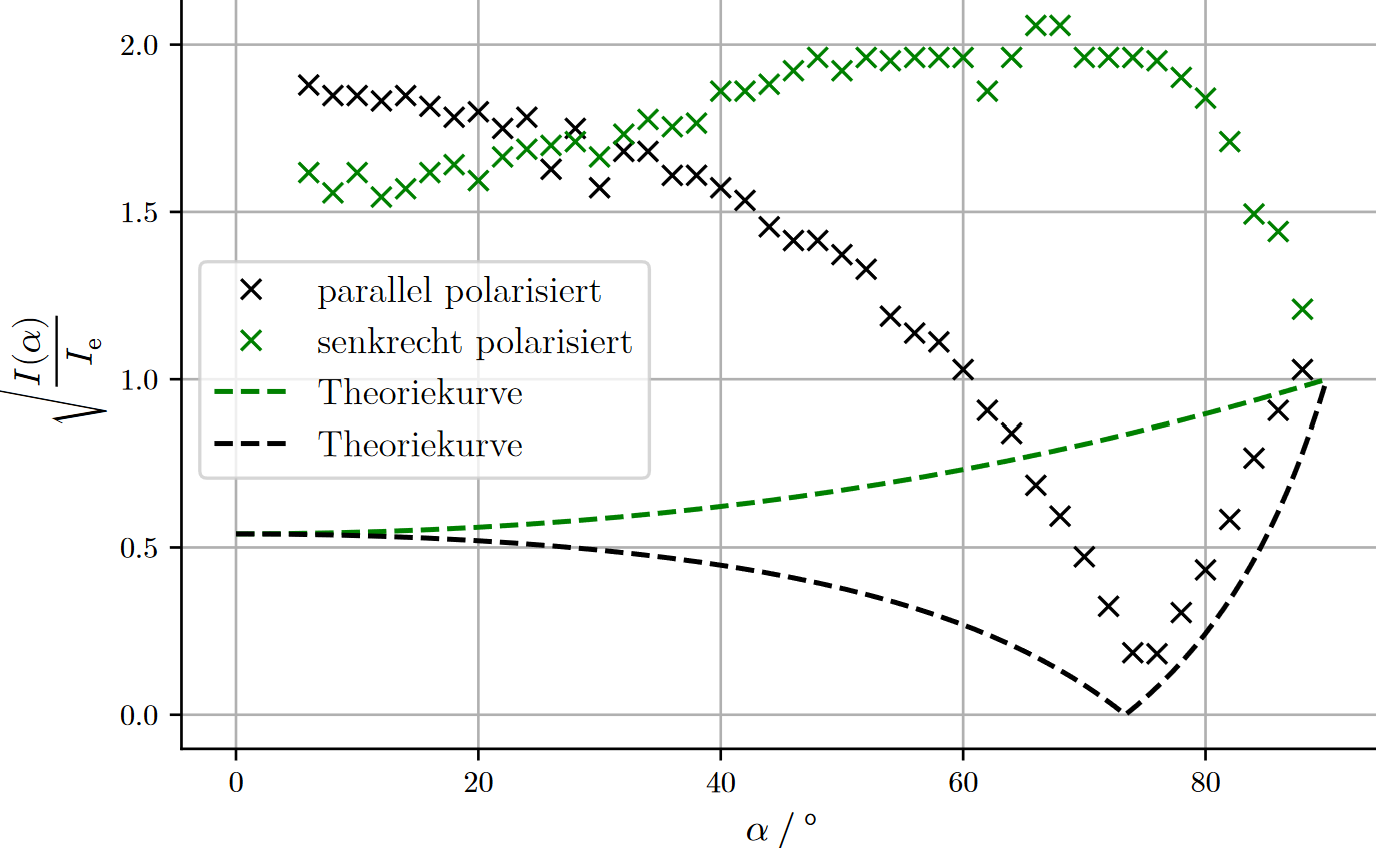
\includegraphics[width=9cm]{plot}
  \caption{Das Verhältnis des reflektierten und einfallenden Stroms gegen den Winkel.}
  \label{plot}
\end{figure}
Aus dem Plot und aus den Messwerten in \autoref{sec:a} ist erkennbar, das der Brewsterwinkel bei ungefähr $\alpha_p=73^\circ$ liegt. Mit \eqref{} ergibt sich 
\begin{equation*}
  n=3.27
\end{equation*}
für den Brechungsindex von Silizium bei Licht mit der Wellenlänge $\lambda=633\ \textrm{nm}$.
